\documentclass{ctexart}
\usepackage{graphicx}
\usepackage{amsmath}
\usepackage{booktabs}
\usepackage[left=2.5cm,right=2.5cm,top=2.5cm,bottom=2.5cm]{geometry}
\begin{document}
\begin{center}
    \Large{电路实验4预习报告}\\
    Leo
    
\end{center}
\section{预习要求}
\subsection{确定实验内容1的电路电阻取值}
实验1要求时间常数$\tau$=0.066ms。根据公式
\begin{equation}
    \tau=RC
\end{equation}
可得电阻取值为
\begin{equation}
    R=\dfrac{\tau}{C}=3k\Omega
\end{equation}
\subsection{按照实验2参数要求,结合自身已有元件参数,设计微分、积分电路。并用Multisim进行仿真,预先测量记录相应的波形及数据}
\subsubsection{积分电路}
设计如图\ref{fig:积分电路}所示的RC电路。设置电源电压幅值$U_S=10V$,频率为$f=25kHz$,电阻为$R=22M\Omega$,电容为$C=10pF$。
\begin{figure}[!ht]
    \centering
    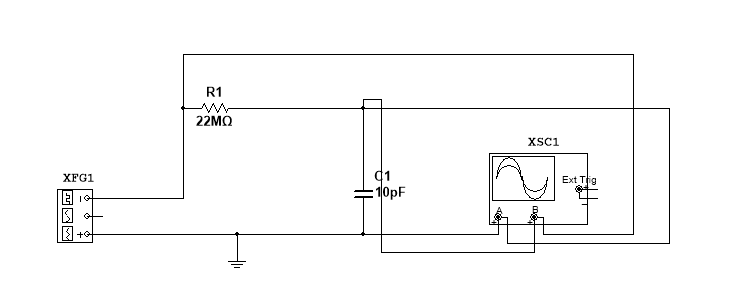
\includegraphics{pic/积分电路.png}
    \caption{积分电路}
    \label{fig:积分电路}
\end{figure}
通过示波器显示如图\ref{fig:示波器1}所示的波形,得到其最大值为901.822mV,最小值为-906.278mV。
\begin{figure}
    \centering
    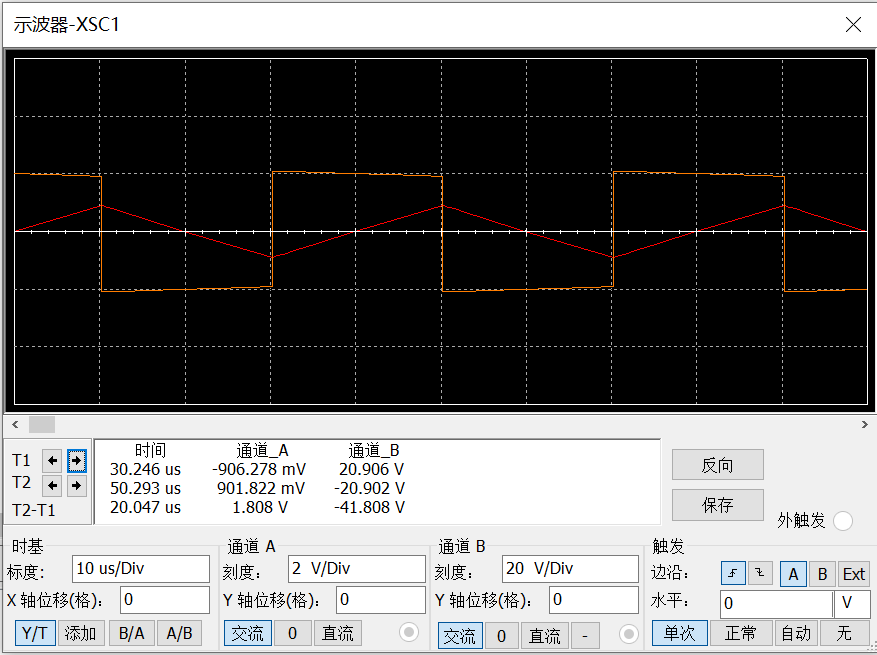
\includegraphics{pic/示波器1.png}
    \caption{示波器1}
    \label{fig:示波器1}
\end{figure}
已知电容的特性为
\begin{equation}
    U_C=\dfrac{1}{C}\int_0^t i(t)dt
\end{equation}
又由于时间常数$\tau$远大于5倍周期,因此在电容电压的每个波形内,电容都没有充分充放电,将输入电压的方波近似为了锯齿波,电阻上的电压占总电压的绝大部分。因此有
\begin{equation}
    U_C=\dfrac{1}{C}\int_0^t i(t)dt =\dfrac{1}{RC}\int _0^t U_s(t)dt
\end{equation}
输出电压的极差
\begin{equation}
    \Delta U_O = 1.808V 
\end{equation}
\begin{equation}
    \dfrac{\Delta U_O}{U_S}=0.181
\end{equation}
\subsection{微分电路}
\begin{figure}
    \centering
    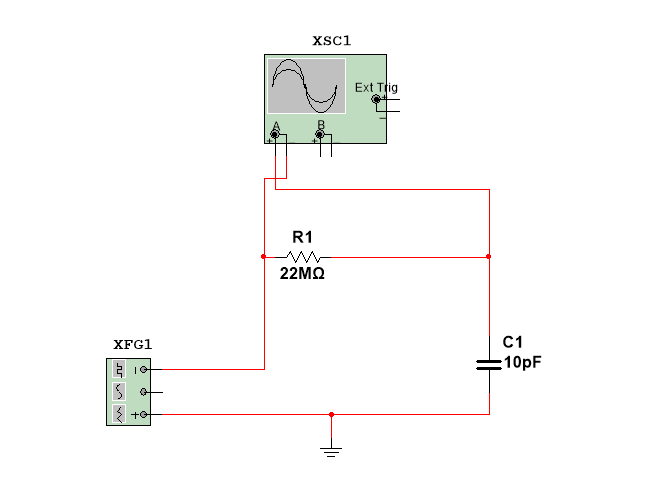
\includegraphics{pic/微分电路.png}
    \caption{微分电路}
    \label{fig:微分电路}
\end{figure}
保持上一步的电路结构,将示波器接到电阻两端,并将电源频率设置为100Hz,此时$\tau$远小于周期T,故在绝大部分时间内$U_C=U_S$,
继而有
\begin{equation}
    U_O(t)=Ri(t)=RC\dfrac{dU_C(t)}{dt}=RC\dfrac{dU_S(t)}{dt}
\end{equation}
\begin{figure}
    \centering
    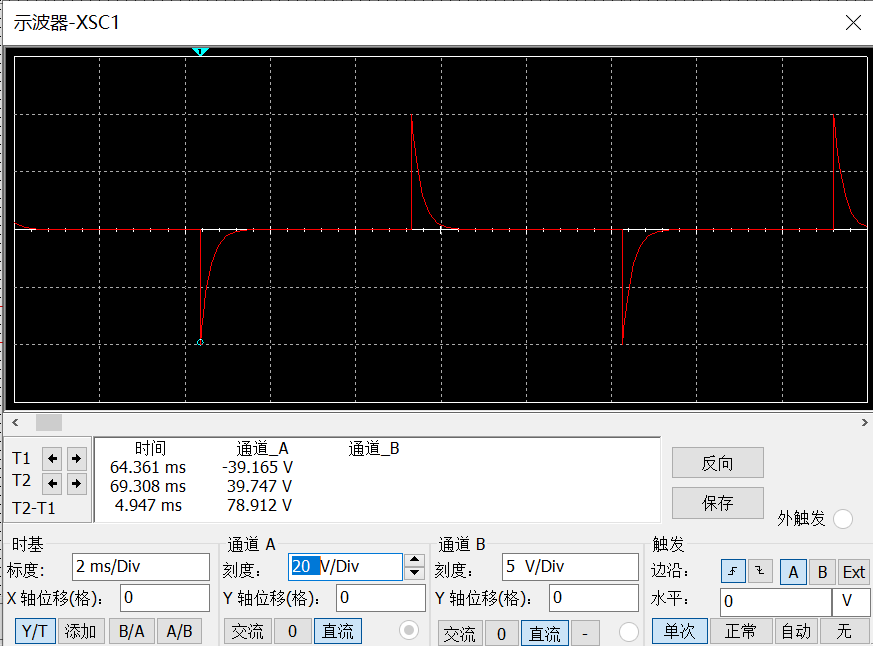
\includegraphics{pic/示波器2.png}
    \caption{示波器2}
    \label{fig:示波器2}
\end{figure}
输出电压的峰峰值
\begin{equation}
    \Delta U_O = 78.912V 
\end{equation}
\begin{equation}
    \dfrac{\Delta U_O}{U_S}=7.891
\end{equation}
因此,只需要测量输出电压再除以时间常数即可求得电压源函数关于时间的微分。但需要注意的是,该等式仅在大约0.1T时间内有效(即图中波形不为零的部分)且计算精度波动较大。

\end{document}
